\documentclass[11pt]{article}
\usepackage[margin=0.75in]{geometry}
\usepackage{amsmath,amssymb}
\usepackage{tikz}
\usepackage{pgfplots}
\usepackage{booktabs}
\usepackage{xcolor}
\usepackage{float}
\usepackage{multicol}

\usetikzlibrary{patterns,decorations.pathmorphing,calc,arrows.meta,positioning,shapes.geometric,decorations.markings}
\pgfplotsset{compat=1.18}

% Brand colors
\definecolor{garnet}{HTML}{73000A}
\definecolor{atlantic}{HTML}{466A9F}
\definecolor{congaree}{HTML}{1F414D}
\definecolor{horseshoe}{HTML}{65780B}
\definecolor{rose}{HTML}{CC2E40}
\definecolor{black90}{HTML}{363636}
\definecolor{black70}{HTML}{5C5C5C}
\definecolor{black50}{HTML}{A2A2A2}
\definecolor{black30}{HTML}{C7C7C7}
\definecolor{honeycomb}{HTML}{A49137}
\definecolor{sandstorm}{HTML}{FFF2E3}
\definecolor{grass}{HTML}{CED318}

% Solar ray color
\definecolor{sunray}{HTML}{FFD700}

\newcommand{\degC}{$^\circ$C}

\title{\textbf{Solar Cooker Design Comparison:\\Types, Principles, and Schematics}}
\author{J.C. Vaught}
\date{\today}

\begin{document}
\maketitle

\section{Overview of Solar Cooker Types}

\begin{table}[H]
\centering
\caption{Comparison of main solar cooker types}
\small
\begin{tabular}{lccccc}
\toprule
\textbf{Type} & \textbf{Max Temp} & \textbf{Efficiency} & \textbf{Cost} & \textbf{Tracking} & \textbf{Best For} \\
\midrule
Box & 150\degC & 25--35\% & \$\$ & None & Baking, stews \\
Parabolic & 370\degC & 50--65\% & \$\$\$ & Frequent & Frying, grilling \\
Panel & 150\degC & 20--30\% & \$ & Occasional & Portable, DIY \\
Evacuated Tube & 280\degC & 40--50\% & \$\$\$\$ & None & Cold climates \\
Hybrid + Storage & 150\degC & 35--55\% & \$\$\$\$ & Varies & Evening cooking \\
\bottomrule
\end{tabular}
\end{table}

%=============================================================================
\section{Type 1: Box Solar Cooker}
%=============================================================================

\subsection{Working Principle}
An insulated box with a glass top creates a greenhouse effect. Sunlight enters through the glass, is absorbed by the black interior, and the trapped heat cooks food slowly at moderate temperatures.

\begin{figure}[H]
\centering
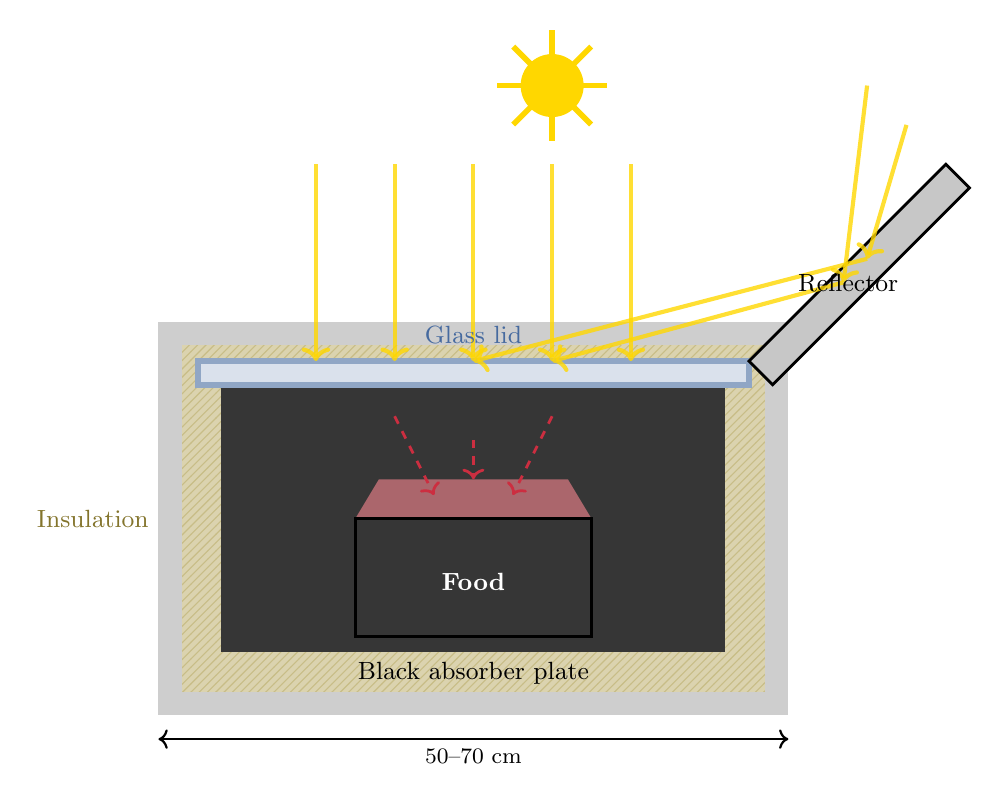
\begin{tikzpicture}[scale=1.0]
    % Outer box
    \fill[black70!30] (0,0) rectangle (8,5);

    % Insulation layer
    \fill[honeycomb!40] (0.3,0.3) rectangle (7.7,4.7);
    \pattern[pattern=north east lines, pattern color=honeycomb!60] (0.3,0.3) rectangle (7.7,4.7);

    % Inner cooking chamber (black)
    \fill[black90] (0.8,0.8) rectangle (7.2,4.2);

    % Glass lid
    \fill[atlantic!20] (0.5,4.2) rectangle (7.5,4.5);
    \draw[line width=2pt, atlantic!60] (0.5,4.2) rectangle (7.5,4.5);

    % Reflector lid (tilted)
    \fill[black30] (7.5,4.5) -- (10,7) -- (10.3,6.7) -- (7.8,4.2) -- cycle;
    \draw[line width=1pt] (7.5,4.5) -- (10,7) -- (10.3,6.7) -- (7.8,4.2) -- cycle;

    % Cooking pot
    \fill[black90] (2.5,1) rectangle (5.5,2.5);
    \fill[garnet!60] (2.5,2.5) -- (2.8,3) -- (5.2,3) -- (5.5,2.5) -- cycle;
    \draw[line width=1pt] (2.5,1) rectangle (5.5,2.5);
    \node[white, font=\small\bfseries] at (4,1.7) {Food};

    % Sun rays - direct
    \foreach \x in {2,3,4,5,6} {
        \draw[->, line width=1.5pt, sunray, opacity=0.8] (\x,7) -- (\x,4.5);
    }

    % Sun rays - from reflector
    \draw[->, line width=1.5pt, sunray, opacity=0.8] (9,8) -- (8.7,5.5);
    \draw[->, line width=1.5pt, sunray, opacity=0.8] (8.7,5.5) -- (5,4.5);
    \draw[->, line width=1.5pt, sunray, opacity=0.8] (9.5,7.5) -- (9,5.8);
    \draw[->, line width=1.5pt, sunray, opacity=0.8] (9,5.8) -- (4,4.5);

    % Heat arrows inside
    \draw[->, line width=1pt, rose, dashed] (4,3.5) -- (4,3);
    \draw[->, line width=1pt, rose, dashed] (3,3.8) -- (3.5,2.8);
    \draw[->, line width=1pt, rose, dashed] (5,3.8) -- (4.5,2.8);

    % Labels
    \node[right, font=\small] at (8,5.5) {Reflector};
    \node[above, font=\small, atlantic] at (4,4.6) {Glass lid};
    \node[left, font=\small, honeycomb!80!black] at (0,2.5) {Insulation};
    \node[below, font=\small] at (4,0.8) {Black absorber plate};

    % Dimensions
    \draw[<->, line width=0.8pt] (0,-0.3) -- (8,-0.3);
    \node[below, font=\footnotesize] at (4,-0.3) {50--70 cm};

    % Sun symbol
    \fill[sunray] (5,8) circle (0.4);
    \foreach \a in {0,45,...,315} {
        \draw[sunray, line width=2pt] (5,8) -- ({5+0.7*cos(\a)},{8+0.7*sin(\a)});
    }

\end{tikzpicture}
\caption{\textbf{Box Solar Cooker} -- Cross-section showing insulated chamber, glass lid, reflector, and cooking pot. Greenhouse effect traps heat inside.}
\end{figure}

\subsection{Key Features}
\begin{itemize}
    \item Double or triple glass glazing reduces heat loss
    \item Black interior maximizes absorption (absorptivity $\alpha > 0.95$)
    \item Insulation (fiberglass, straw, or foam) minimizes conduction losses
    \item Reflector lid increases solar input by 30--50\%
    \item No tracking required; works for 4--6 hours without adjustment
\end{itemize}

%=============================================================================
\newpage
\section{Type 2: Parabolic Solar Cooker}
%=============================================================================

\subsection{Working Principle}
A parabolic reflector concentrates sunlight to a focal point where the cooking pot is placed. The concentrated rays can achieve very high temperatures for frying and grilling.

\begin{figure}[H]
\centering
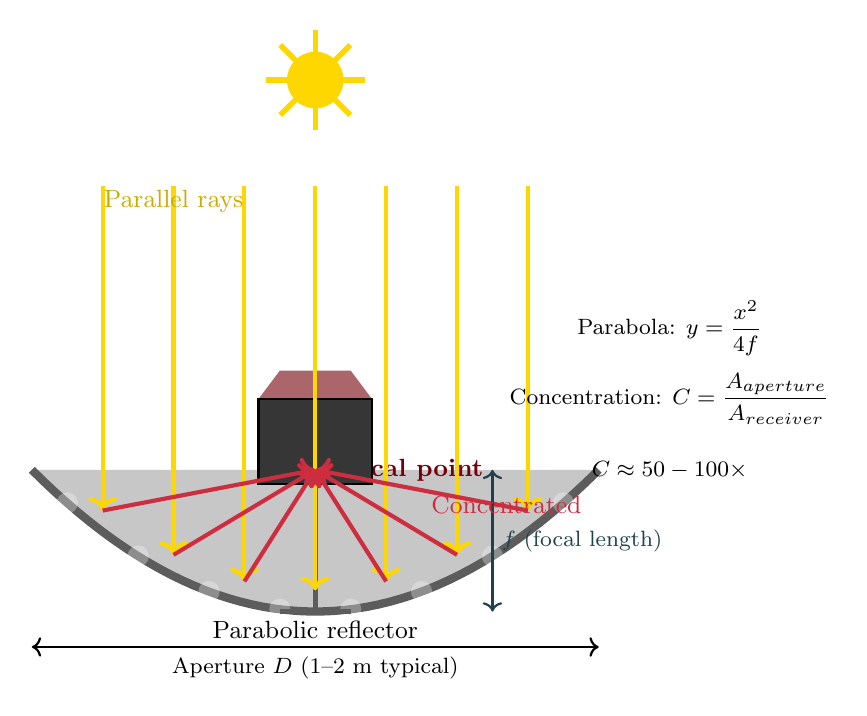
\begin{tikzpicture}[scale=0.9]
    % Parabolic dish (y = x^2/4f, f=2)
    \draw[line width=3pt, black70, fill=black30] plot[domain=-4:4, samples=50] (\x, {0.125*\x*\x});

    % Reflective surface indication
    \foreach \x in {-3.5,-2.5,...,3.5} {
        \fill[white, opacity=0.3] (\x, {0.125*\x*\x}) circle (0.15);
    }

    % Focal point
    \fill[garnet] (0,2) circle (0.15);
    \node[right, font=\small\bfseries, garnet] at (0.2,2) {Focal point};

    % Cooking pot at focus
    \fill[black90] (-0.8,1.8) rectangle (0.8,3);
    \fill[garnet!60] (-0.8,3) -- (-0.5,3.4) -- (0.5,3.4) -- (0.8,3) -- cycle;
    \draw[line width=1pt] (-0.8,1.8) rectangle (0.8,3);

    % Support structure
    \draw[line width=2pt, black70] (0,2) -- (0,0);
    \draw[line width=2pt, black70] (-0.5,0) -- (0.5,0);

    % Sun rays coming in parallel
    \foreach \x in {-3,-2,-1,0,1,2,3} {
        \draw[->, line width=1.5pt, sunray] (\x,6) -- (\x,{0.125*\x*\x + 0.3});
    }

    % Reflected rays to focus
    \draw[->, line width=1.5pt, rose] (-3,{0.125*9 + 0.3}) -- (0,2);
    \draw[->, line width=1.5pt, rose] (-2,{0.125*4 + 0.3}) -- (0,2);
    \draw[->, line width=1.5pt, rose] (-1,{0.125*1 + 0.3}) -- (0,2);
    \draw[->, line width=1.5pt, rose] (1,{0.125*1 + 0.3}) -- (0,2);
    \draw[->, line width=1.5pt, rose] (2,{0.125*4 + 0.3}) -- (0,2);
    \draw[->, line width=1.5pt, rose] (3,{0.125*9 + 0.3}) -- (0,2);

    % Focal length indicator
    \draw[<->, line width=0.8pt, congaree] (2.5,0) -- (2.5,2);
    \node[right, font=\footnotesize, congaree] at (2.5,1) {$f$ (focal length)};

    % Aperture diameter
    \draw[<->, line width=0.8pt] (-4,-0.5) -- (4,-0.5);
    \node[below, font=\footnotesize] at (0,-0.5) {Aperture $D$ (1--2 m typical)};

    % Sun symbol
    \fill[sunray] (0,7.5) circle (0.4);
    \foreach \a in {0,45,...,315} {
        \draw[sunray, line width=2pt] (0,7.5) -- ({0.7*cos(\a)},{7.5+0.7*sin(\a)});
    }

    % Labels
    \node[below, font=\small] at (0,0) {Parabolic reflector};
    \node[above, font=\small, sunray!80!black] at (-2,5.5) {Parallel rays};
    \node[right, font=\small, rose] at (1.5,1.5) {Concentrated};

    % Equation
    \node[font=\footnotesize] at (5,4) {Parabola: $y = \dfrac{x^2}{4f}$};
    \node[font=\footnotesize] at (5,3) {Concentration: $C = \dfrac{A_{aperture}}{A_{receiver}}$};
    \node[font=\footnotesize] at (5,2) {$C \approx 50-100\times$};

\end{tikzpicture}
\caption{\textbf{Parabolic Solar Cooker} -- Parallel sun rays are reflected to a focal point where the pot is placed. High concentration ratio enables temperatures $>$300\degC.}
\end{figure}

\subsection{Key Features}
\begin{itemize}
    \item Concentration ratio 50--100$\times$ achieves 300--400\degC
    \item Optimal focal length $f = D/4$ for maximum angle tolerance
    \item Requires tracking every 15--30 minutes
    \item Deep dish designs (focus inside dish) are safer
    \item Can fry, grill, and boil water in minutes
\end{itemize}

%=============================================================================
\newpage
\section{Type 3: Panel Solar Cooker (CooKit Style)}
%=============================================================================

\subsection{Working Principle}
Multiple flat reflective panels direct sunlight onto a cooking pot, which is often placed inside a transparent heat-resistant bag or under an inverted glass bowl to create a mini-greenhouse.

\begin{figure}[H]
\centering
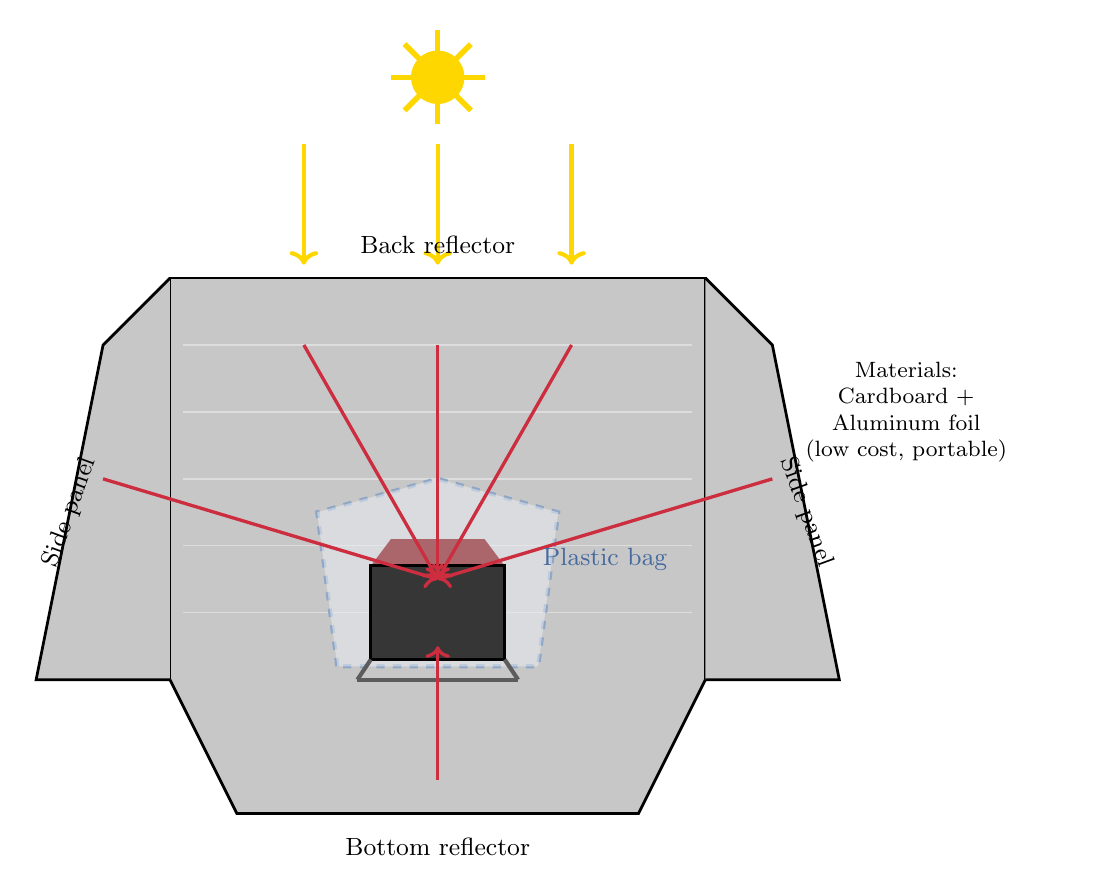
\begin{tikzpicture}[scale=0.85]
    % Back panel (large)
    \fill[black30] (-4,0) -- (-4,6) -- (4,6) -- (4,0) -- cycle;
    \draw[line width=1pt] (-4,0) -- (-4,6) -- (4,6) -- (4,0);

    % Side panels (angled)
    \fill[black30] (-4,0) -- (-6,0) -- (-5,5) -- (-4,6) -- cycle;
    \draw[line width=1pt] (-4,0) -- (-6,0) -- (-5,5) -- (-4,6);

    \fill[black30] (4,0) -- (6,0) -- (5,5) -- (4,6) -- cycle;
    \draw[line width=1pt] (4,0) -- (6,0) -- (5,5) -- (4,6);

    % Bottom panel
    \fill[black30] (-4,0) -- (-3,-2) -- (3,-2) -- (4,0) -- cycle;
    \draw[line width=1pt] (-4,0) -- (-3,-2) -- (3,-2) -- (4,0);

    % Reflective surface lines
    \foreach \y in {1,2,3,4,5} {
        \draw[white, opacity=0.4, line width=0.5pt] (-3.8,\y) -- (3.8,\y);
    }

    % Cooking pot with transparent bag
    \begin{scope}[shift={(0,0.5)}]
        % Plastic bag outline
        \draw[line width=1.5pt, atlantic!60, dashed] (-1.5,-0.3) -- (-1.8,2) -- (0,2.5) -- (1.8,2) -- (1.5,-0.3) -- cycle;
        \fill[atlantic!10, opacity=0.5] (-1.5,-0.3) -- (-1.8,2) -- (0,2.5) -- (1.8,2) -- (1.5,-0.3) -- cycle;

        % Black pot inside
        \fill[black90] (-1,-0.2) rectangle (1,1.2);
        \fill[garnet!60] (-1,1.2) -- (-0.7,1.6) -- (0.7,1.6) -- (1,1.2) -- cycle;
        \draw[line width=1pt] (-1,-0.2) rectangle (1,1.2);

        % Wire stand
        \draw[line width=1.5pt, black70] (-1.2,-0.5) -- (-1,-0.2);
        \draw[line width=1.5pt, black70] (1.2,-0.5) -- (1,-0.2);
        \draw[line width=1.5pt, black70] (-1.2,-0.5) -- (1.2,-0.5);
    \end{scope}

    % Sun rays
    \foreach \x in {-2,0,2} {
        \draw[->, line width=1.5pt, sunray] (\x,8) -- (\x,6.2);
    }

    % Reflected rays from back panel
    \draw[->, line width=1.2pt, rose] (-2,5) -- (0,1.5);
    \draw[->, line width=1.2pt, rose] (0,5) -- (0,1.5);
    \draw[->, line width=1.2pt, rose] (2,5) -- (0,1.5);

    % Reflected rays from side panels
    \draw[->, line width=1.2pt, rose] (-5,3) -- (0,1.5);
    \draw[->, line width=1.2pt, rose] (5,3) -- (0,1.5);

    % Reflected rays from bottom
    \draw[->, line width=1.2pt, rose] (0,-1.5) -- (0,0.5);

    % Labels
    \node[font=\small] at (0,6.5) {Back reflector};
    \node[font=\small, rotate=70] at (-5.5,2.5) {Side panel};
    \node[font=\small, rotate=-70] at (5.5,2.5) {Side panel};
    \node[font=\small, atlantic] at (2.5,1.8) {Plastic bag};
    \node[font=\small] at (0,-2.5) {Bottom reflector};

    % Sun
    \fill[sunray] (0,9) circle (0.4);
    \foreach \a in {0,45,...,315} {
        \draw[sunray, line width=2pt] (0,9) -- ({0.7*cos(\a)},{9+0.7*sin(\a)});
    }

    % Material note
    \node[font=\footnotesize, text width=4cm, align=center] at (7,4) {Materials:\\Cardboard +\\Aluminum foil\\(low cost, portable)};

\end{tikzpicture}
\caption{\textbf{Panel Solar Cooker (CooKit)} -- Flat reflective panels surround a pot in a transparent bag. Simple, cheap, and highly portable.}
\end{figure}

\subsection{Key Features}
\begin{itemize}
    \item Made from cardboard and aluminum foil (\$5--20)
    \item Folds flat for transport; weighs $<$1 kg
    \item Transparent bag/bowl creates greenhouse effect around pot
    \item Temperatures reach 120--150\degC
    \item Requires repositioning every 1--2 hours
    \item Ideal for slow cooking rice, beans, stews
\end{itemize}

%=============================================================================
\newpage
\section{Type 4: Evacuated Tube Solar Cooker}
%=============================================================================

\subsection{Working Principle}
Vacuum-insulated glass tubes absorb solar radiation with minimal heat loss. Heat is transferred to a cooking chamber via heat pipes or circulating fluid. Works even in cold weather.

\begin{figure}[H]
\centering
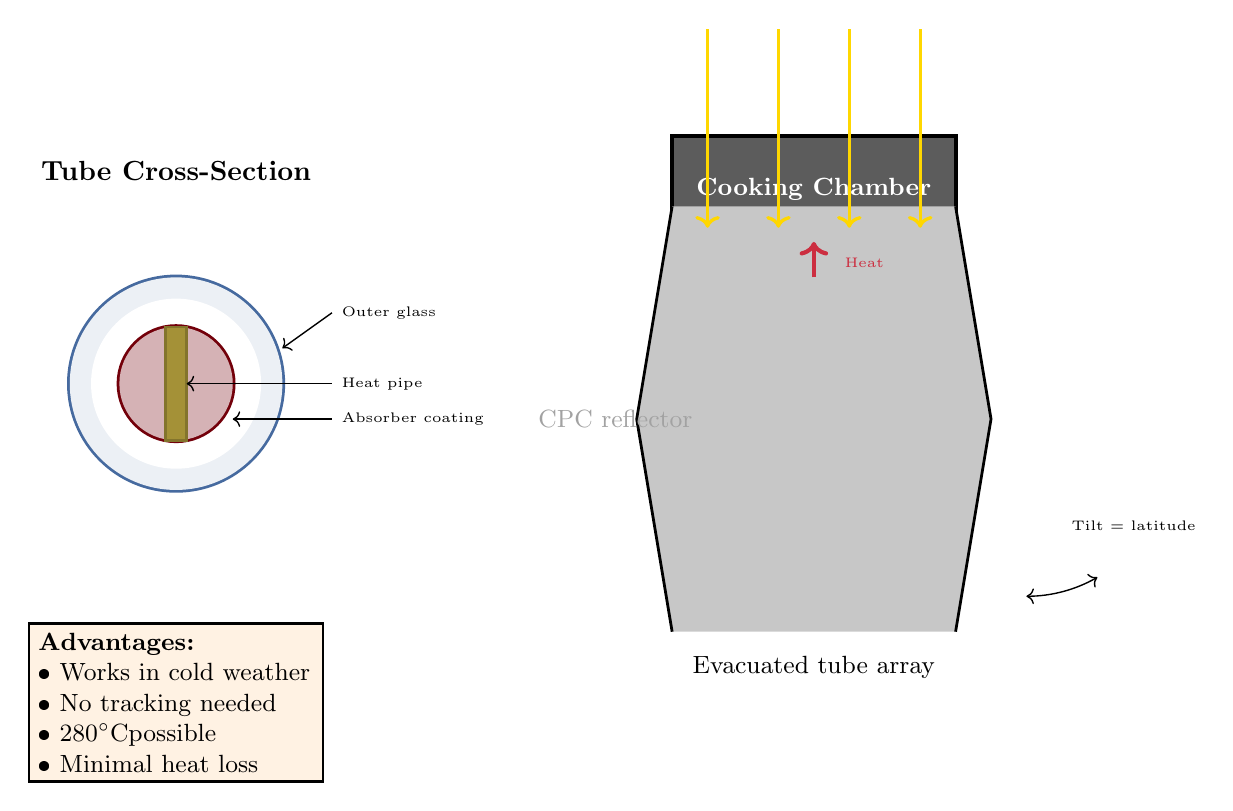
\begin{tikzpicture}[scale=0.9]
    % Single evacuated tube cross-section (large detail)
    \begin{scope}[shift={(-5,3)}]
        \node[font=\bfseries] at (0,3) {Tube Cross-Section};

        % Outer glass tube
        \draw[line width=2pt, atlantic] (0,0) circle (1.5);
        \fill[atlantic!10] (0,0) circle (1.5);

        % Vacuum space
        \fill[white] (0,0) circle (1.2);
        \node[font=\tiny] at (0,0.6) {Vacuum};

        % Inner tube with absorber
        \draw[line width=2pt, garnet] (0,0) circle (0.8);
        \fill[garnet!30] (0,0) circle (0.8);

        % Heat pipe (copper)
        \fill[honeycomb] (-0.15,-0.8) rectangle (0.15,0.8);
        \draw[line width=1pt, honeycomb!80!black] (-0.15,-0.8) rectangle (0.15,0.8);

        % Labels
        \draw[<-, line width=0.5pt] (1.5,0.5) -- (2.2,1);
        \node[right, font=\tiny] at (2.2,1) {Outer glass};

        \draw[<-, line width=0.5pt] (0.8,-0.5) -- (2.2,-0.5);
        \node[right, font=\tiny] at (2.2,-0.5) {Absorber coating};

        \draw[<-, line width=0.5pt] (0.15,0) -- (2.2,0);
        \node[right, font=\tiny] at (2.2,0) {Heat pipe};
    \end{scope}

    % Full system view
    \begin{scope}[shift={(3,0)}]
        % Cooking chamber/manifold
        \fill[black70] (-1,5) rectangle (3,6.5);
        \draw[line width=1.5pt] (-1,5) rectangle (3,6.5);
        \node[white, font=\small\bfseries] at (1,5.75) {Cooking Chamber};

        % Evacuated tubes (array)
        \foreach \x in {-0.5,0.5,1.5,2.5} {
            % Tube body
            \fill[atlantic!20] (\x-0.25,0) rectangle (\x+0.25,5);
            \draw[line width=1pt, atlantic] (\x-0.25,0) -- (\x-0.25,5);
            \draw[line width=1pt, atlantic] (\x+0.25,0) -- (\x+0.25,5);

            % Rounded bottom
            \fill[atlantic!20] (\x,0) ellipse (0.25 and 0.15);
            \draw[line width=1pt, atlantic] (\x,0) ellipse (0.25 and 0.15);

            % Inner absorber
            \fill[garnet!40] (\x-0.12,0.2) rectangle (\x+0.12,4.8);

            % Heat pipe to manifold
            \draw[line width=2pt, honeycomb] (\x,4.8) -- (\x,5);
        }

        % Reflector behind tubes
        \fill[black30] (-1,-0.5) -- (-1.5,2.5) -- (-1,5.5) -- (3,5.5) -- (3.5,2.5) -- (3,-0.5) -- cycle;
        \draw[line width=1pt] (-1,-0.5) -- (-1.5,2.5) -- (-1,5.5);
        \draw[line width=1pt] (3,-0.5) -- (3.5,2.5) -- (3,5.5);

        % Sun rays
        \foreach \x in {-0.5,0.5,1.5,2.5} {
            \draw[->, line width=1.2pt, sunray] (\x,8) -- (\x,5.2);
        }

        % Heat flow arrows
        \draw[->, line width=1.5pt, rose] (1,4.5) -- (1,5);
        \node[right, font=\tiny, rose] at (1.3,4.7) {Heat};

        % Tilt angle
        \draw[<->, line width=0.5pt] (4,0) arc (270:300:2);
        \node[right, font=\tiny] at (4.5,1) {Tilt = latitude};

        % Labels
        \node[font=\small] at (1,-1) {Evacuated tube array};
        \node[font=\small, black50] at (-1.8,2.5) {CPC reflector};
    \end{scope}

    % Performance box
    \node[draw, line width=1pt, fill=sandstorm, text width=3.5cm, font=\small, align=left] at (-5,-1.5) {
        \textbf{Advantages:}\\
        • Works in cold weather\\
        • No tracking needed\\
        • 280\degC possible\\
        • Minimal heat loss
    };

\end{tikzpicture}
\caption{\textbf{Evacuated Tube Solar Cooker} -- Vacuum insulation minimizes heat loss. Heat pipes transfer energy to cooking chamber. Works in cloudy/cold conditions.}
\end{figure}

\subsection{Key Features}
\begin{itemize}
    \item Vacuum between glass layers eliminates convection/conduction losses
    \item Selective absorber coating: high absorptivity ($\alpha > 0.92$), low emissivity ($\varepsilon < 0.08$)
    \item Compound Parabolic Concentrator (CPC) reflector boosts collection
    \item Can reach 280\degC; works even below freezing
    \item Higher cost but excellent performance in marginal conditions
\end{itemize}

%=============================================================================
\newpage
\section{Type 5: Hybrid/Indirect Cooker with Thermal Storage}
%=============================================================================

\subsection{Working Principle}
Solar collector is separate from cooking area. Heat transfer fluid (oil or water) or phase change material (PCM) stores thermal energy for cooking after sunset or indoors.

\begin{figure}[H]
\centering
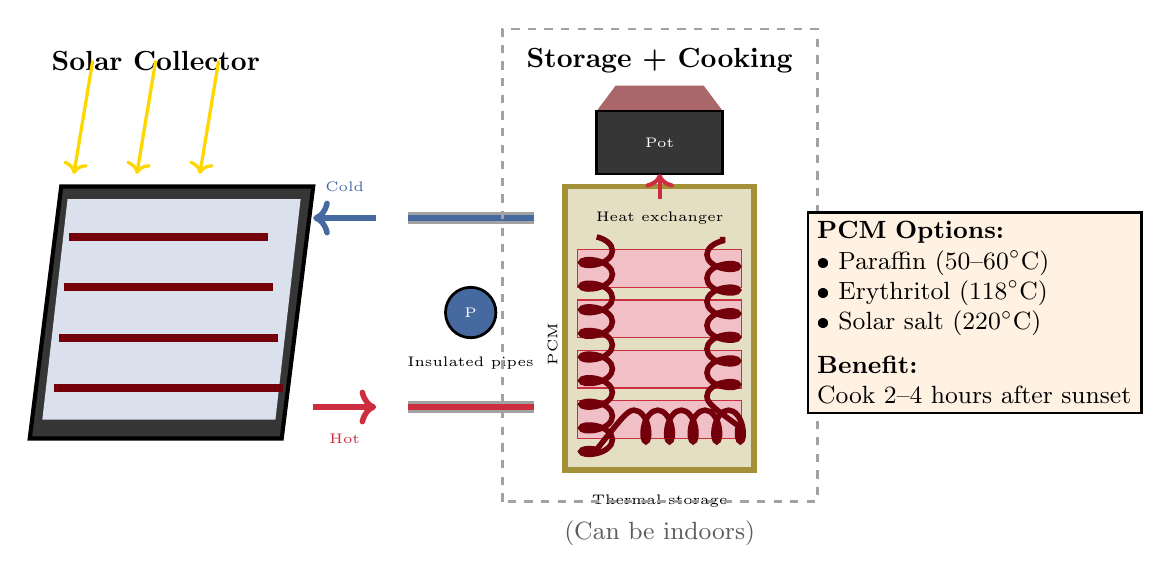
\begin{tikzpicture}[scale=0.8]
    % Solar collector (outdoor)
    \begin{scope}[shift={(-4,0)}]
        \node[font=\bfseries] at (0,6) {Solar Collector};

        % Collector panel (tilted)
        \fill[black90] (-2,0) -- (-1.5,4) -- (2.5,4) -- (2,0) -- cycle;
        \draw[line width=1.5pt] (-2,0) -- (-1.5,4) -- (2.5,4) -- (2,0) -- cycle;

        % Glass cover
        \fill[atlantic!20] (-1.8,0.3) -- (-1.4,3.8) -- (2.3,3.8) -- (1.9,0.3) -- cycle;

        % Absorber tubes
        \foreach \y in {0.8,1.6,2.4,3.2} {
            \draw[line width=3pt, garnet] ({-1.7+0.1*\y},\y) -- ({2.1-0.1*\y},\y);
        }

        % Sun rays
        \foreach \x in {-1,0,1} {
            \draw[->, line width=1.2pt, sunray] (\x,6) -- (\x-0.3,4.2);
        }

        % Flow arrows
        \draw[->, line width=2pt, rose] (2.5,0.5) -- (3.5,0.5);
        \draw[<-, line width=2pt, atlantic] (2.5,3.5) -- (3.5,3.5);

        \node[font=\tiny, rose] at (3,0) {Hot};
        \node[font=\tiny, atlantic] at (3,4) {Cold};
    \end{scope}

    % Insulated pipes
    \draw[line width=4pt, black50] (0,0.5) -- (2,0.5);
    \draw[line width=4pt, black50] (0,3.5) -- (2,3.5);
    \draw[line width=2pt, rose] (0,0.5) -- (2,0.5);
    \draw[line width=2pt, atlantic] (0,3.5) -- (2,3.5);
    \node[font=\tiny, rotate=0] at (1,1.2) {Insulated pipes};

    % Thermal storage tank
    \begin{scope}[shift={(4,0)}]
        \node[font=\bfseries] at (0,6) {Storage + Cooking};

        % Storage tank
        \fill[honeycomb!30] (-1.5,-0.5) rectangle (1.5,4);
        \draw[line width=2pt, honeycomb] (-1.5,-0.5) rectangle (1.5,4);

        % PCM layers
        \foreach \y in {0,0.8,1.6,2.4} {
            \fill[rose!30] (-1.3,\y) rectangle (1.3,{\y+0.6});
            \draw[line width=0.5pt, rose] (-1.3,\y) rectangle (1.3,{\y+0.6});
        }
        \node[font=\tiny, rotate=90] at (-1.7,1.5) {PCM};

        % Heat exchanger coils
        \draw[line width=2pt, garnet, decorate, decoration={coil, aspect=0.5, segment length=3mm, amplitude=2mm}]
            (-1,3.2) -- (-1,0.2) -- (1,0.2) -- (1,3.2);

        % Cooking pot on top
        \fill[black90] (-1,4.2) rectangle (1,5.2);
        \fill[garnet!60] (-1,5.2) -- (-0.7,5.6) -- (0.7,5.6) -- (1,5.2) -- cycle;
        \draw[line width=1pt] (-1,4.2) rectangle (1,5.2);
        \node[white, font=\tiny] at (0,4.7) {Pot};

        % Heat flow up
        \draw[->, line width=1.5pt, rose] (0,3.8) -- (0,4.2);

        % Labels
        \node[font=\tiny] at (0,-1) {Thermal storage};
        \node[font=\tiny] at (0,3.5) {Heat exchanger};

        % Can be indoors indicator
        \draw[dashed, line width=1pt, black50] (-2.5,-1) rectangle (2.5,6.5);
        \node[font=\small, black70] at (0,-1.5) {(Can be indoors)};
    \end{scope}

    % Pump
    \fill[atlantic] (1,2) circle (0.4);
    \draw[line width=1pt] (1,2) circle (0.4);
    \node[white, font=\tiny] at (1,2) {P};

    % Performance note
    \node[draw, line width=1pt, fill=sandstorm, text width=4cm, font=\small, align=left] at (9,2) {
        \textbf{PCM Options:}\\
        • Paraffin (50--60\degC)\\
        • Erythritol (118\degC)\\
        • Solar salt (220\degC)\\[0.5em]
        \textbf{Benefit:}\\
        Cook 2--4 hours after sunset
    };

\end{tikzpicture}
\caption{\textbf{Hybrid Solar Cooker with Thermal Storage} -- Separate collector and cooking unit connected by heat transfer loop. PCM stores heat for evening cooking.}
\end{figure}

\subsection{Key Features}
\begin{itemize}
    \item Cooking can happen indoors, away from collector
    \item Phase Change Materials (PCM) store latent heat
    \item Extends cooking 2--4 hours after sunset
    \item Higher complexity and cost, but most versatile
    \item Best for community kitchens and consistent daily use
\end{itemize}

%=============================================================================
\newpage
\section{Design Comparison Summary}
%=============================================================================

\begin{figure}[H]
\centering
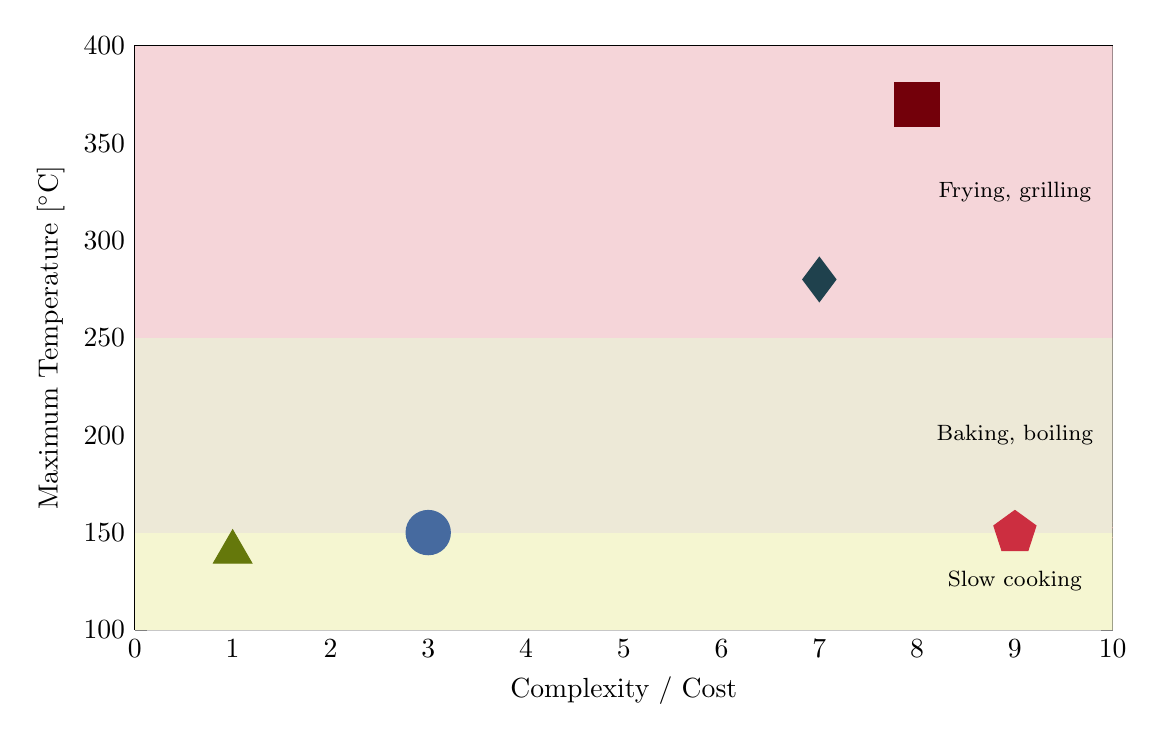
\begin{tikzpicture}
\begin{axis}[
    width=14cm,
    height=9cm,
    xlabel={Complexity / Cost},
    ylabel={Maximum Temperature [\degC]},
    xmin=0, xmax=10,
    ymin=100, ymax=400,
    grid=both,
    grid style={line width=0.2pt, draw=black30},
    legend pos=south east,
    legend style={font=\small},
]

% Data points for each type
\addplot[only marks, mark=*, mark size=8pt, color=atlantic] coordinates {(3, 150)};
\addplot[only marks, mark=square*, mark size=8pt, color=garnet] coordinates {(8, 370)};
\addplot[only marks, mark=triangle*, mark size=8pt, color=horseshoe] coordinates {(1, 140)};
\addplot[only marks, mark=diamond*, mark size=8pt, color=congaree] coordinates {(7, 280)};
\addplot[only marks, mark=pentagon*, mark size=8pt, color=rose] coordinates {(9, 150)};

% Labels
\node[right, font=\small, atlantic] at (axis cs:3.3, 150) {Box};
\node[right, font=\small, garnet] at (axis cs:8.3, 370) {Parabolic};
\node[right, font=\small, horseshoe] at (axis cs:1.3, 140) {Panel};
\node[right, font=\small, congaree] at (axis cs:7.3, 280) {Evacuated Tube};
\node[right, font=\small, rose] at (axis cs:9.3, 150) {Hybrid+PCM};

% Temperature zones
\fill[grass!20] (axis cs:0,100) rectangle (axis cs:10,150);
\fill[honeycomb!20] (axis cs:0,150) rectangle (axis cs:10,250);
\fill[rose!20] (axis cs:0,250) rectangle (axis cs:10,400);

\node[font=\footnotesize] at (axis cs:9, 125) {Slow cooking};
\node[font=\footnotesize] at (axis cs:9, 200) {Baking, boiling};
\node[font=\footnotesize] at (axis cs:9, 325) {Frying, grilling};

\end{axis}
\end{tikzpicture}
\caption{Solar cooker types mapped by complexity/cost vs. maximum temperature capability.}
\end{figure}

\section{Recommendations by Use Case}

\begin{table}[H]
\centering
\begin{tabular}{lll}
\toprule
\textbf{Use Case} & \textbf{Recommended Type} & \textbf{Reason} \\
\midrule
Backpacking/emergency & Panel (CooKit) & Light, cheap, foldable \\
Home daily cooking & Box cooker & Reliable, no tracking, safe \\
High-temp cooking (frying) & Parabolic & Only option for $>$250\degC \\
Cold/cloudy climates & Evacuated tube & Works in poor conditions \\
Evening/indoor cooking & Hybrid + PCM & Thermal storage capability \\
Community kitchen & Hybrid + PCM & Scalable, consistent output \\
\bottomrule
\end{tabular}
\end{table}

\end{document}
